
\section{图表}

我们也可以插入图片(figure),比如 \cref{fig:attention}。
\begin{figure}[htpb]
    \centering
    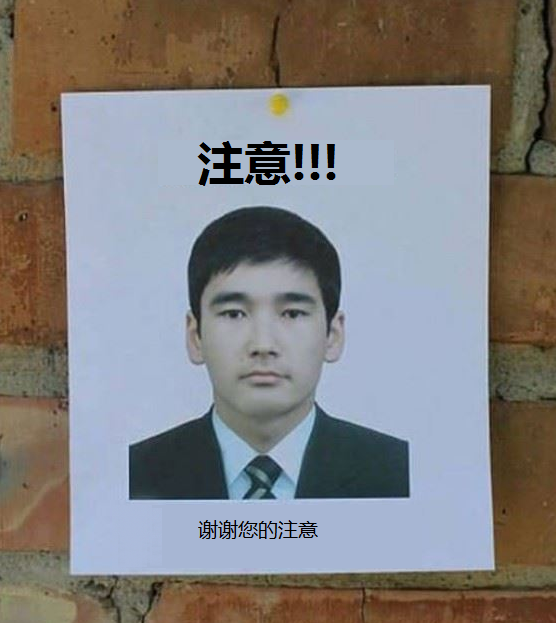
\includegraphics[width=0.6\linewidth]{pics/thanks-for-your-attention.png}
    \caption{中国某市某繁华街区十字路口附近的墙上张贴的启事}
    \label{fig:attention}
\end{figure}
写的时候尽量使用 \code`label` 与 \code`cref` 交叉引用的方式来书写。
避免依靠图、表的位置来描述。
即多使用 \code`如 \cref{xxx} 所示`
而避免使用 \code`如下图所示`
这样的语言。

要插入一张表(table),就使用 \code`table` 环境。
你可以用 Word 做好表导出成图片再引用进来(如 \cref{tab:wordtab})。
也可以在 \LaTeX\ 中编写表格(如 \cref{tab:latextab}),
其实也很简单。

\begin{table}[htpb]
    \centering
    \caption{%
        这张表是用 Google Doc 制作、再作为图片的形式导入进来的。
    }
    \label{tab:wordtab}
    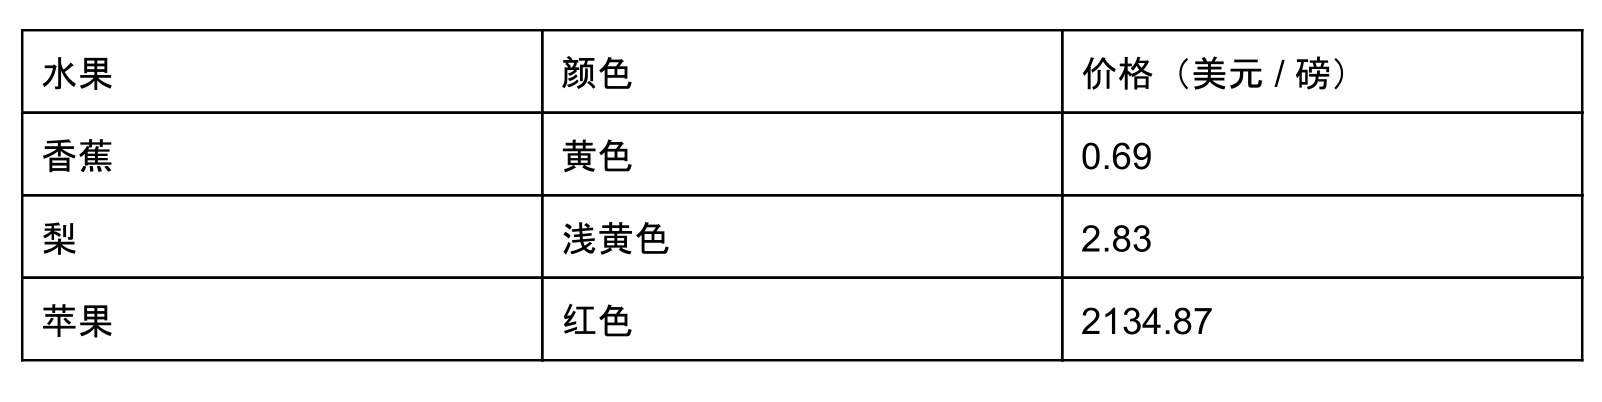
\includegraphics[width=10cm]{pics/fruit-specs.png}
\end{table}

\begin{table}[htpb]
    \centering
    \caption{%
        这张表是直接使用 \LaTeX\ 编写的。
    }
    \label{tab:latextab}
    \begin{tabular}{clr} % 三列,对齐方式分别为:中C 左L 右R
        \toprule
        水果 & 颜色   & 价格(美元/磅) \\
        \midrule
        香蕉 & 黄色   & 0.69            \\
        梨   & 浅黄色 & 2.83            \\
        苹果 & 红色   & 2134.87         \\
        \botrule
    \end{tabular}
\end{table}

